\begin{event}{GAP in Algebraic Research Summer School in Aachen}{GAP in Algebraic Research}{Aachen, Germany, 19th-22nd of November 2018}{USTAN}{41}{1}{https://lbfm-rwth.github.io/gap-in-algebraic-research-2018/}

\textbf{Main goals.} The aim of this ``summer'' school was 
to give an overview of different applications of GAP in mathematical research. 

\textbf{ODK implication.} Alexander Konovalov was one of the instructors. 
Costs \pounds 560.

\textbf{Event summary.} The speakers presented their areas of research, 
the functionality that is available in GAP to investigate these areas 
computationally, and guided participants through these tools during the 
accompanying hands-on programming lab sessions.

\textbf{Results and impact.} Alexander Konovalov
gave an introductory GAP Tutorial based on the 
Software Carpentry lesson ``Programming with GAP''
(\url{https://doi.org/10.5281/zenodo.597073}),
demonstrated GAP Jupyter notebooks and parallel 
distributed calculations using the SCSCP package.
The format of this part of the school's programme
followed the Software Carpentry teaching approaches.
In particular, we collected the feedback on minute
cards after each of the half-day sessions. Some quotes
from the feedback written by the learners:

- Nice step-by-step introduction

- Good organisation of materials and presentation

- The content are quite well organised 

- Idea with stickers is cool. This really makes asking questions easier

- I really like the use of stickers as tools for asking for help and give feedback

- I really liked the tutorial, well explained, and differences between listing on a group elements or a group G!!!

- Appropriate speed

- Started from the beginning, easy to follow

- The session was understandable

- I learned a lot of interesting 'short' commands

- Lots of shortcuts - I am very lazy

- Very useful tips on optimising the working process (autocompletion etc)

- Many nice details

- "Real-life" example of application (average order of group elements) that demonstrate necessary syntax =)

- Good to solve a simple problem, not only technical details

- Programming with a goal in mind

- Very informative and useful

- Like presentation of different packages - also interesting for people knowing GAP

- Excellent the Jupyter notebook!! Incredible! I would like to see more about this application.

- References to "modern" interfaces like Jupyter instead of command line

- Some interesting tricks for people who already know GAP

- The graphical applications were awesome!

\begin{figure}[ht]
  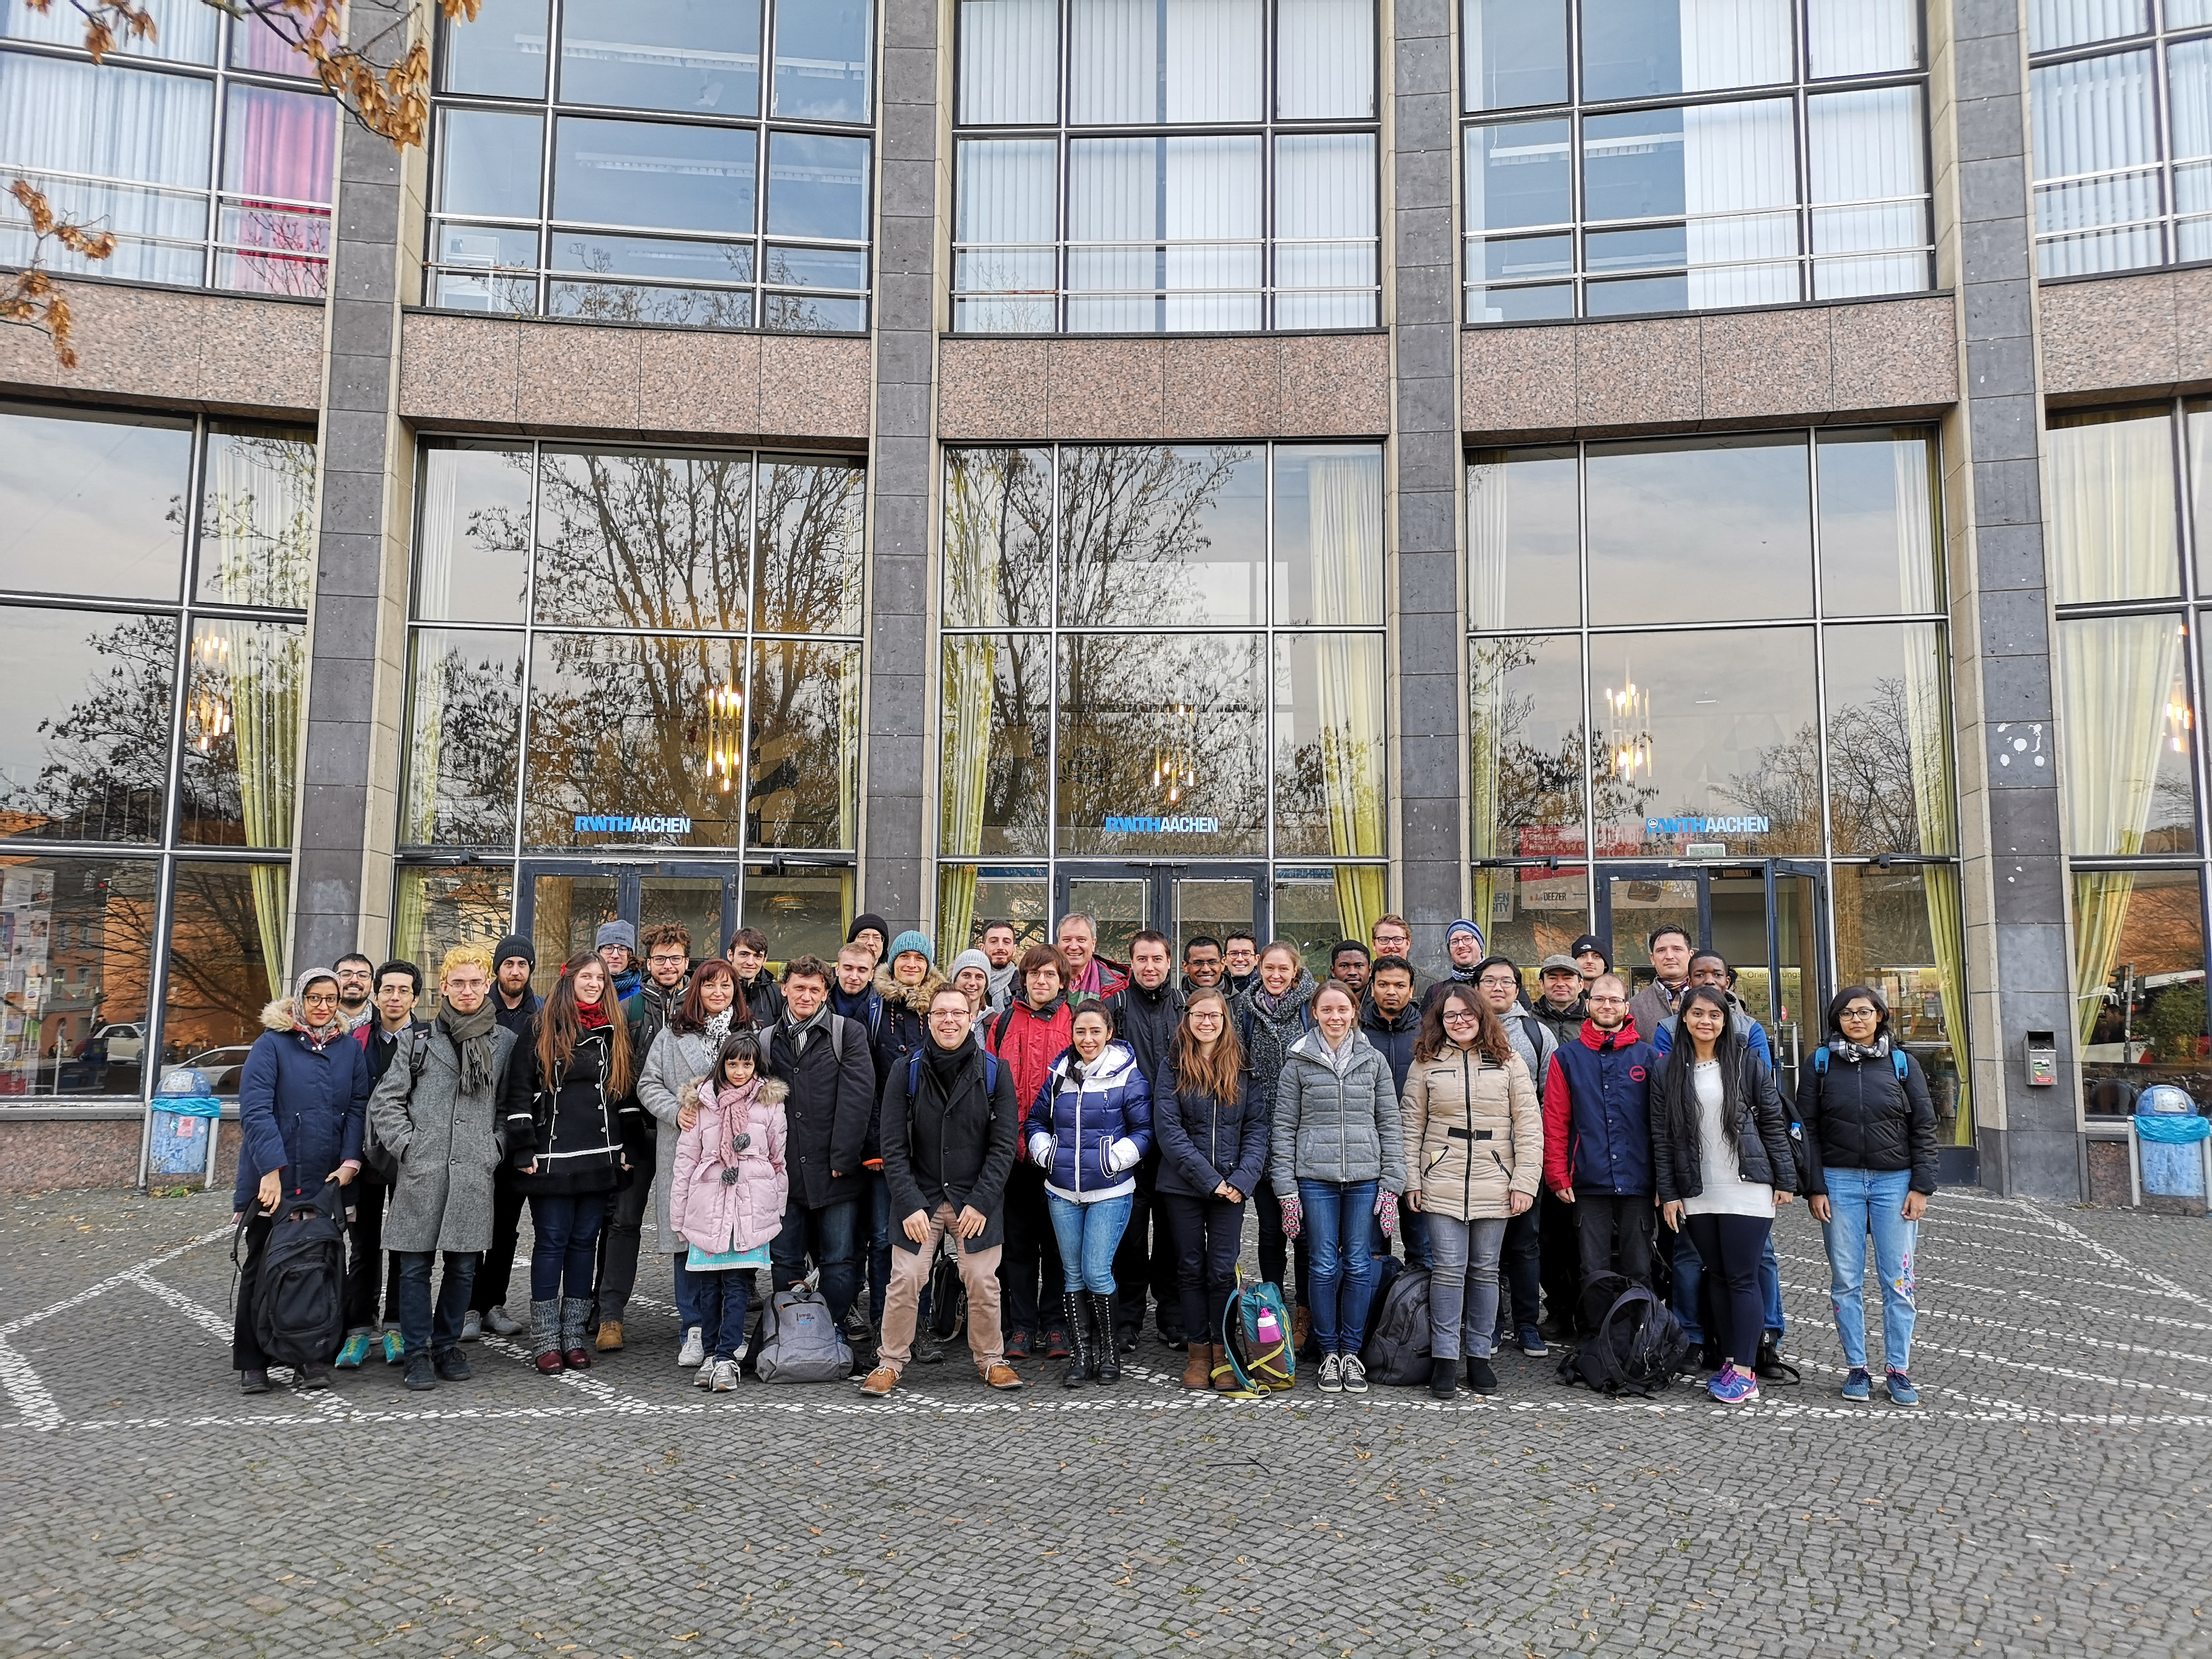
\includegraphics[width=\textwidth]{Aachen_school_2018}
  \caption*{GAP in Algebraic Research Summer School, Aachen, Germany}
\end{figure}

\end{event}
